\section{Robustness of \cref{fig:map}}
\label{sec:map}

\Cref{fig:map} pairs every whole-image call with every split of the same item by the same model in our data: all 40 LegendSpot drawings and all floor-plan items (including those used to write the prompt and set thresholds) with the tiles of the 44 px recipe and its fixed-grid counterpart, and the natural images with same-scale $2 \times 2$ tiles against the upsampled whole image. The models are the eight sweep models of \cref{tab:experiments}, with Gemini 3.8 at its three budgets. A pair is a split that never zooms out if every tile has at least the whole-image call's $S$, and otherwise one that zooms out; the grouping uses geometry only. Each pair is binned by the whole-image call's $S$ and number of targets, and a cell with fewer than 10 pairs is left blank. Intervals resample images, and source drawings for the mosaics, so that pairs of one image across models and areas move together. \Cref{tab:mapci} gives every cell with its interval; \cref{fig:map-models} and \cref{fig:map-data} split the map by model and by data set, and \cref{fig:map-cxcy} recomputes it reading only points written with the requested \texttt{cx} and \texttt{cy} keys (\cref{sec:coords}). For $S$ between 1.5 and 3, the gain of \cref{fig:map}(a) pooled over targets is +0.13 for Gemini 3.8, +0.14 for Gemma 4, +0.13 for Qwen3-VL, +0.09 for Claude Sonnet 4.6 and +0.08 for Claude Sonnet 5.5, against $-0.02$ for GPT-5.4, +0.03 for GPT-5.6 and +0.03 for Gemini 2.5. In every version the conclusions of \cref{sec:safe} hold: cells with $S < 1.5$ gain most, and the cells of splits that zoom out are negative. Of the 91 cells of \cref{fig:map-models}, none is significantly below zero; the lowest are Claude Sonnet 5.5's at $S \ge 3$ ($-0.14$ and $-0.12$).

\begin{table}[t]
\centering
\footnotesize
\setlength{\tabcolsep}{2.5pt}
\begin{adjustbox}{max width=\linewidth}\begin{tabular}{lcccrc}
\toprule
Split & Targets & $S$ & Pairs & Mean & 95\% interval \\
\midrule
\inputrows{generated/figH_ci.tex}
\bottomrule
\end{tabular}\end{adjustbox}
\caption{Every cell of \cref{fig:map} with its 95\% bootstrap interval (images resampled; mosaics by source drawing).}
\label{tab:mapci}
\end{table}

\begin{figure*}[t]
\centering
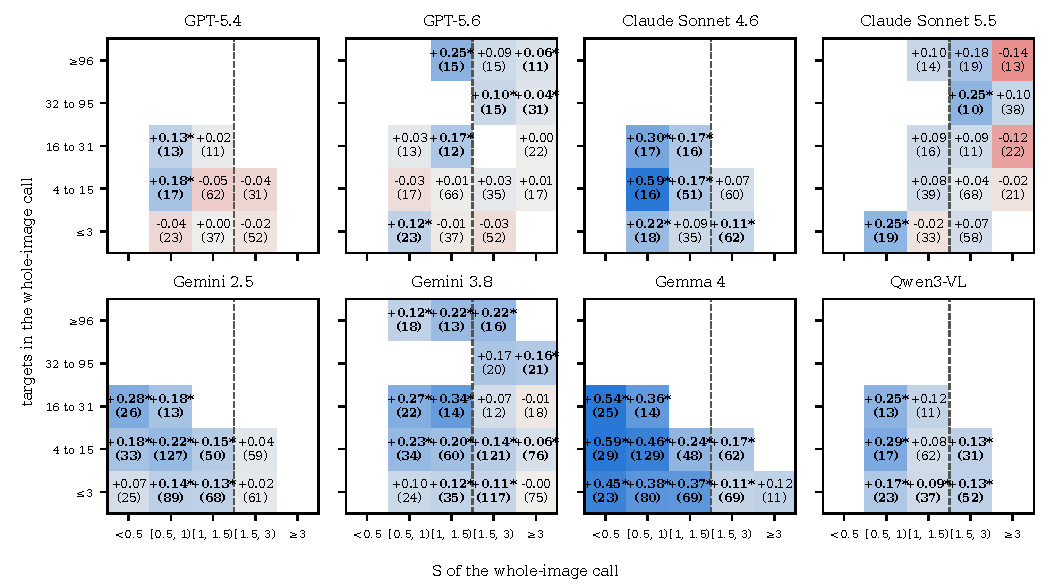
\includegraphics[width=\textwidth]{figures_x/figH_models.pdf}
\caption{\Cref{fig:map}(a), splits that never zoom out, for each of the eight models with tiles in our data. Colour scale as in \cref{fig:map}; cells with fewer than 10 pairs are blank; ${}^\ast$ and bold: 95\% interval excludes 0.}
\label{fig:map-models}
\end{figure*}

\begin{figure*}[t]
\centering
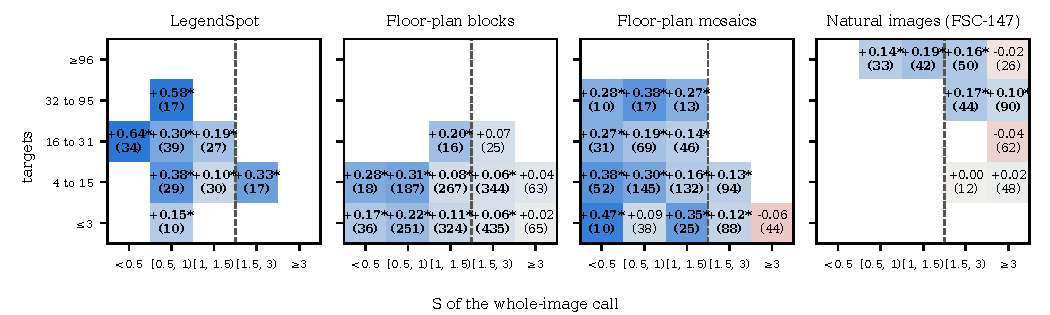
\includegraphics[width=\textwidth]{figures_x/figH_data.pdf}
\caption{\Cref{fig:map}(a) for each data set; cells and markers as in \cref{fig:map-models}.}
\label{fig:map-data}
\end{figure*}

\begin{figure*}[t]
\centering
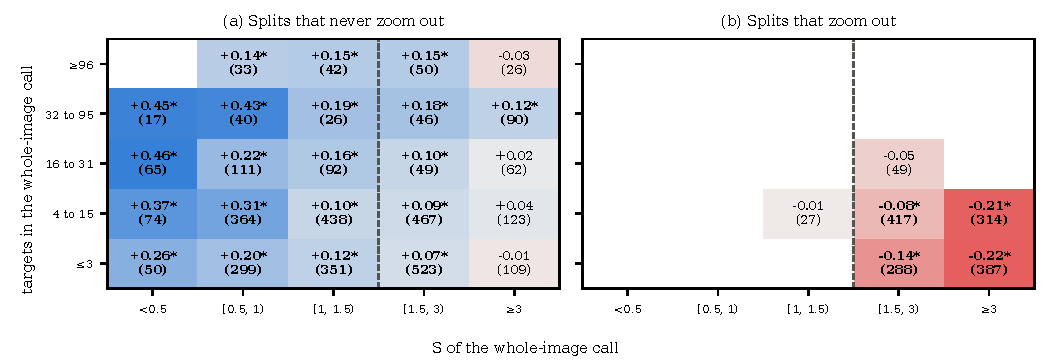
\includegraphics[width=0.9\textwidth]{figures_x/figH_cxcy.pdf}
\caption{\Cref{fig:map} reading only points written with \texttt{cx} and \texttt{cy} keys, which changes some Gemini 3.8 answers.}
\label{fig:map-cxcy}
\end{figure*}
